\documentclass[a4paper,english,10pt]{report}


%\usepackage[french]{babel}
\usepackage[utf8]{inputenc}		% french special caracters (é, è, à, ...)
\usepackage[pdftex]{graphicx}				% to include figure in the document
\usepackage[footnotesize]{caption}      	% caption of table and figure in footnote size
\usepackage{color}                     			% texte en couleurs
\usepackage{subfig}					% allow the use of subfigure in the figure environment
\usepackage{fancyhdr}				% change header and footer
\usepackage{hyperref} 				% make hyperref in the pdf document
\usepackage{geometry}  				% change de geometry of the page
%\usepackage{eurosym}				% use of euro symbol
%\usepackage{floatflt}   				% for floating figure
\usepackage{multirow}
\usepackage{fancyvrb}                   		% pour afficher du code
%\usepackage{amsmath}				% math package
\usepackage{sidecap}				% caption at le left or right side of the figures
%\usepackage{lettrine} 				% emploi de lettrine au debut du chapitre
\usepackage{url}
\usepackage{makeidx}
\usepackage{wrapfig}

\geometry{a4paper,tmargin=3cm,bmargin=2.5cm,lmargin=4cm,rmargin=3cm}
\pagestyle{headings}
\fancyfoot[C]{  \thepage \ }
\bibliographystyle{plain}
\makeindex


%==========================pour les images================================
\graphicspath{{images/graphes/},{images/diagrammes/},
{images/illustrations/}, {images/}}
\DeclareGraphicsExtensions{.jpg,.png, .tiff, .pdf}

%==========================numérotations==================================
\setcounter{tocdepth}{1}                % affiche jusqu'aux susubsections dans toc
\setcounter{secnumdepth}{3}             % chapitres et sections numrots
\setlength{\tolerance}{1000}             % tolrance pour l'espace entre les mots

%==========================pour les couleurs===============================
\definecolor{coolRed}{RGB}{223,0,0}
\definecolor{coolBlue}{rgb}{0.2,0,0.5}
\definecolor{coolSection}{RGB}{50,109,50}
%\definecolor{coolSection}{RGB}{64, 127, 0}
\definecolor{red}{RGB}{255,0,0}
\definecolor{coolSubSection}{RGB}{0,0,0}
\definecolor{coolYellow}{RGB}{254,203,1}
\definecolor{coolGreen}{RGB}{22,109,15}

%=======================en-tête et pieds de page==================================

\pagestyle{fancy}
\fancyhf{}
\fancyhead[L]{\leftmark}
\fancyfoot[R]{\thepage}

%==================== DOCUMENT =================================


\begin{document}
\title{How to digitalized an entire maize root system to create a R-SWMS input file}
\author{Guillaume Lobet\\ \small{Earth and Life Institute, Université catholique de Louvain}}

\maketitle
\tableofcontents

\chapter{Introduction}

\section{General principle}

The general principle of this method is to acquired an R-SWMS input file from a rhizotron grown plant.
The method is divided in three steps:

\begin{enumerate}
\item Scan the root system
\item Digitalize the roots
\item Create the input file
\end{enumerate}

Once the input file is created it be directly used as an input file for the R-SWMS model \cite{Javaux08}.\\

We tested the method with 15-days old maize plants. These plants presented several advantages for the methods:

\begin{itemize}
\item they had thick roots
\item they did not have too much roots
\item but they already had all type of roots (principal, seminal, crown and laterals)
\end{itemize}

The method might not be suitable for plant having thinner roots or for older plants as the manipulation time required for some of the steps might increase dramatically.
%
%\begin{figure}[htbp]
%\begin{center}
%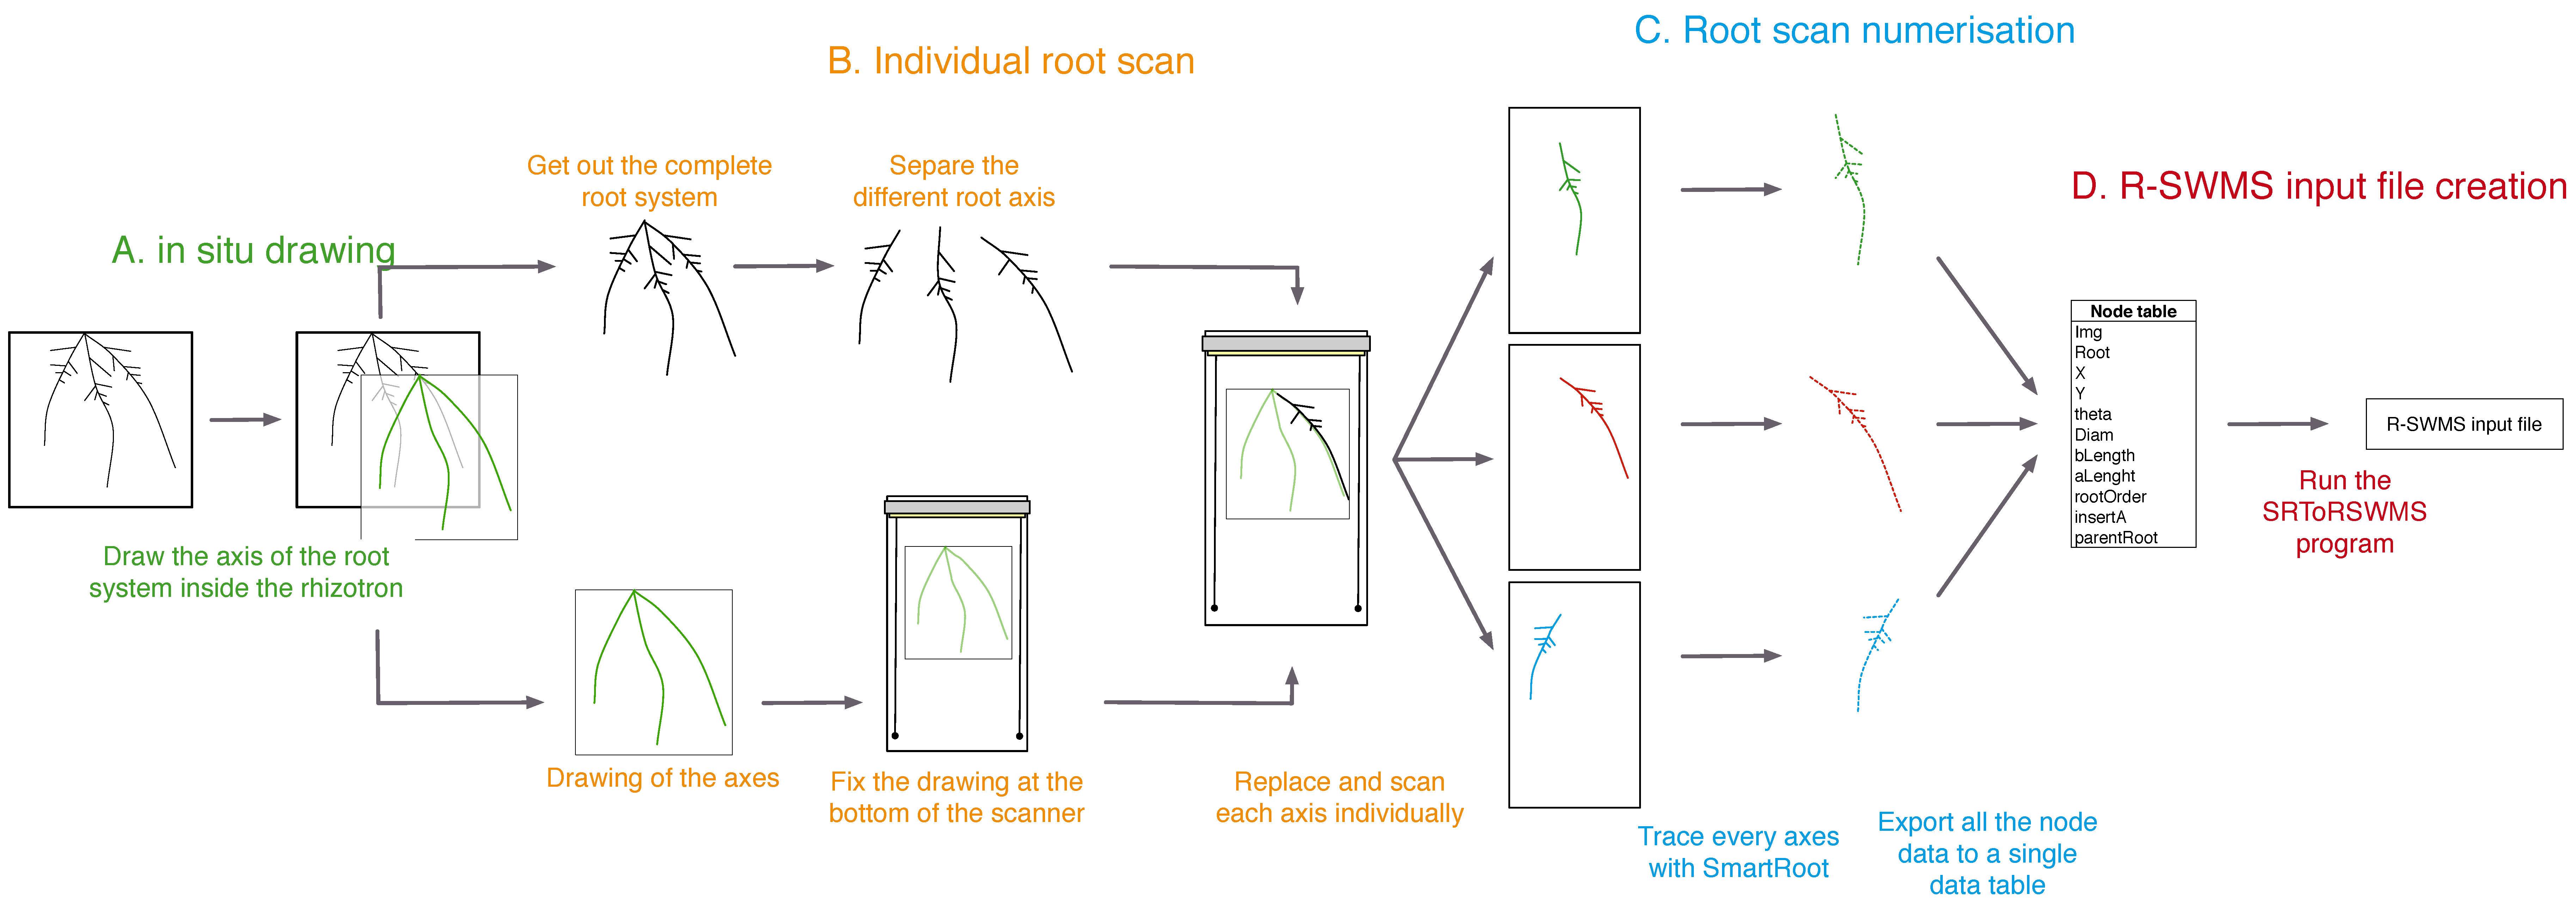
\includegraphics[width=\textheight, angle=90]{rhizo_to_rswms.pdf}
%\caption[Complete data workflow]{\textbf{Data worflow:} From the plant inside the rhizotron to the r-SWMS input file.}
%\label{complete_workflow}
%\end{center}
%\end{figure}

\section{Required material}

\begin{table}[htdp]
\begin{tabular}{p{0.5\linewidth}l}
\textbf{Root drawing:} & transparent film \\
& permanent marker \\
& tape \\ \\ 
\textbf{Root scan:} & flat-bed scanner \\
& scissors \\ \\ 
\textbf{Root digitalization:} & \href{http://rsb.info.nih.gov/ij/index.html}{ImageJ} \\
& \href{http://www.uclouvain.be/en-smartroot}{SmartRoot} \\
& SQL database (Access or MySQL) \\ \\ 
\textbf{R-SWMS input file creation:} & SRToRSWMS.jar \\
\end{tabular}
\end{table}%

%%%%%%%%%%%%%%%%%%%%%%

\chapter{From a rhizotron grown plant to scanned roots}

\section{Principle}

Two type of root images can be obtained from a rhizotron experiment: hand drawing and scanning. The had drawing had the advantage to conserve the geographic information of the root system, but present a poor level of detail. On the other hand, the root scan shows all the roots, but not in the same position as they were in the rhizotron. More over, a scan of a complete root system usually present a lot of overlapping region, leading to bias in the root system analysis.

The method we propose used these two types of image at the same time to acquire a geographically correct, highly detailed root dataset:

\begin{enumerate}
\item Trace the root axis on a transparent film
\item Fix the film with the drawing at the bottom of the scanner
\item Take the root system out of the rhizotron, clean it and separate the different root axis
\item Replace the cut axis on the drawing fixed in the scanner and scan them individually
\end{enumerate}

This method generate on root scan per root axis, with a correct geographic position and a high level of detail.

\begin{figure}[h!]
\begin{center}
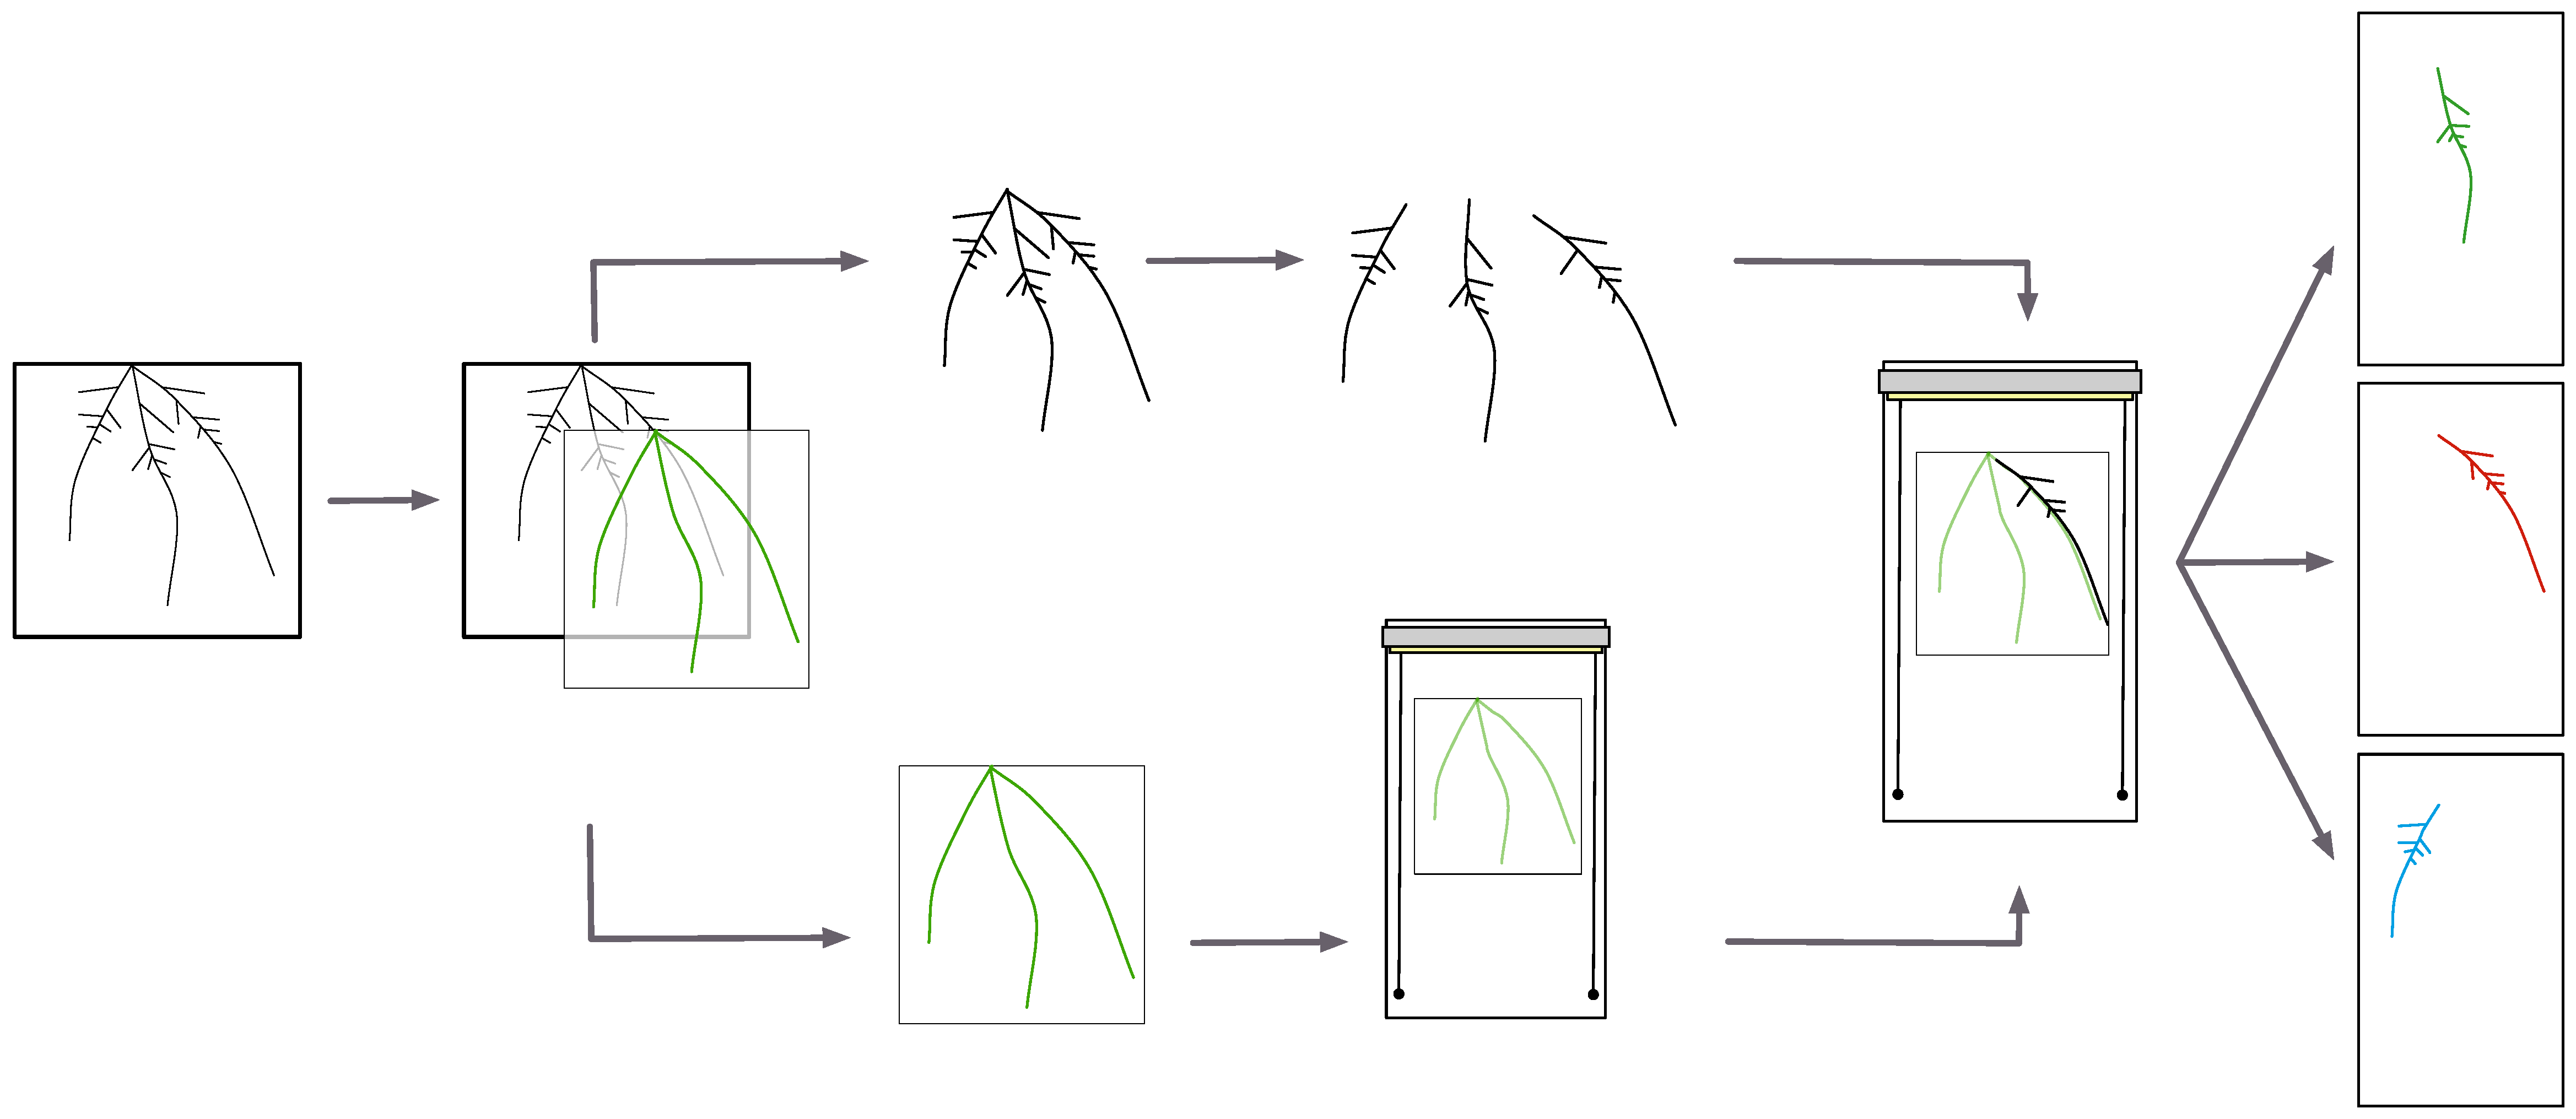
\includegraphics[width=\linewidth]{indiv_root_scan.pdf}
\caption[From a rhizotron grown plant to scanned roots]{\textbf{From a rhizotron grown plant to scanned roots.}}
\label{indiv_root_scan}
\end{center}
\end{figure}

\section{Plant culture}

Plant were grown in thin transparent boxes (rhizotron, fig. \ref{rhizotron}) during two weeks. At this time the plants reached the  fully expanded leaves stage. They root systems had principal, seminal and crown axes (naming according to \cite{Hochholdinger04}) and had a maximal depth between 300 and 500 mm.


\begin{figure}[h]
\centering
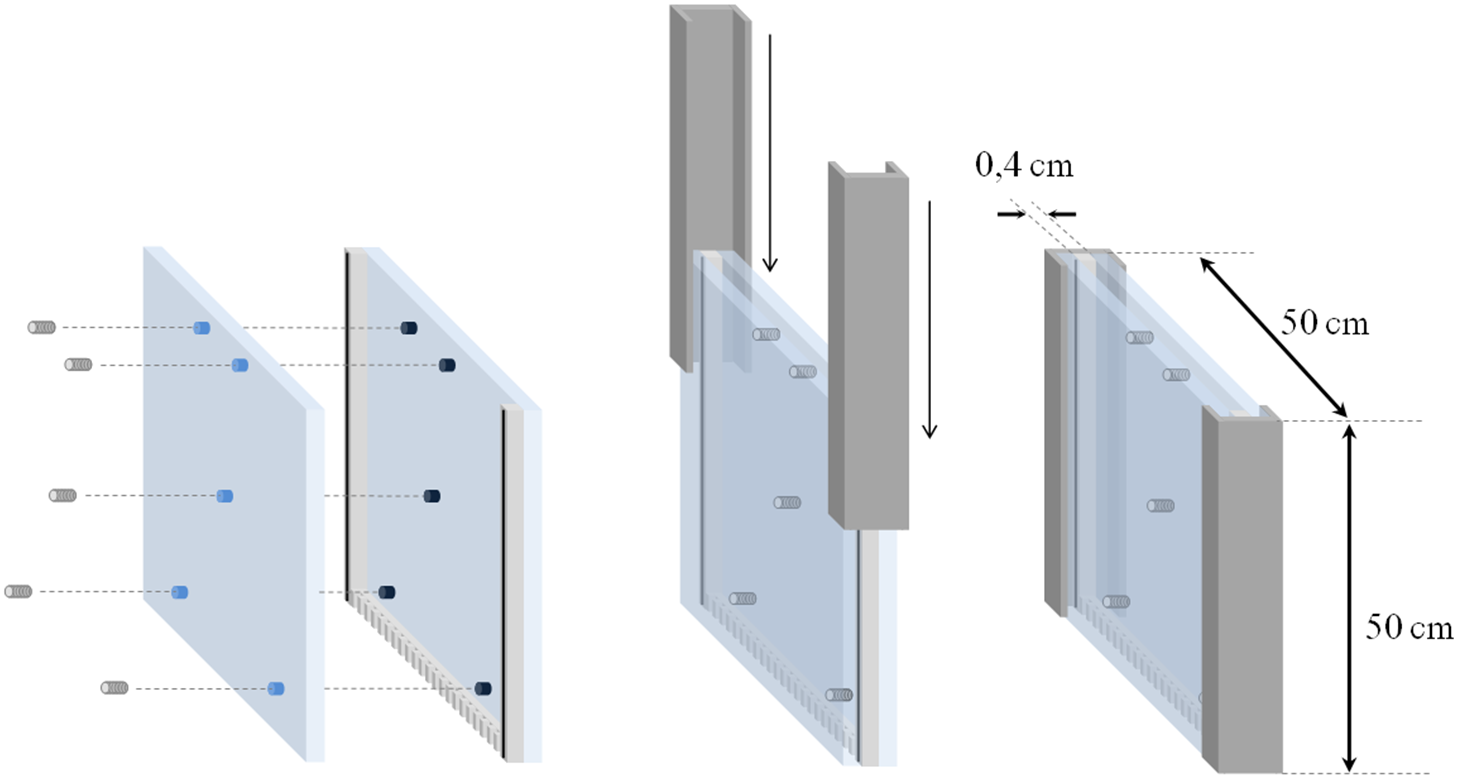
\includegraphics[width=0.6\textwidth]{petits_rhiz}
\caption[Rhizotron]{\textbf{Rhizotrons.} The rhizotron had two transparent sides and an internal volume of 4 x 500 x 500 mm$^3$}
\label{rhizotron}
\end{figure}

\section{Tracing the root axis}

Before tacking the plant out of the rhizotrons, draw on a transparent film the different root axis (fig. \ref{insitu}). \\

For this, it is important to use a color that will not be seen on the root scan (as the drawing will be scanned with the root). Use light colors such as green or yellow, and avoid colors such as red of blue.\\


\begin{figure}[htbp]
\begin{center}
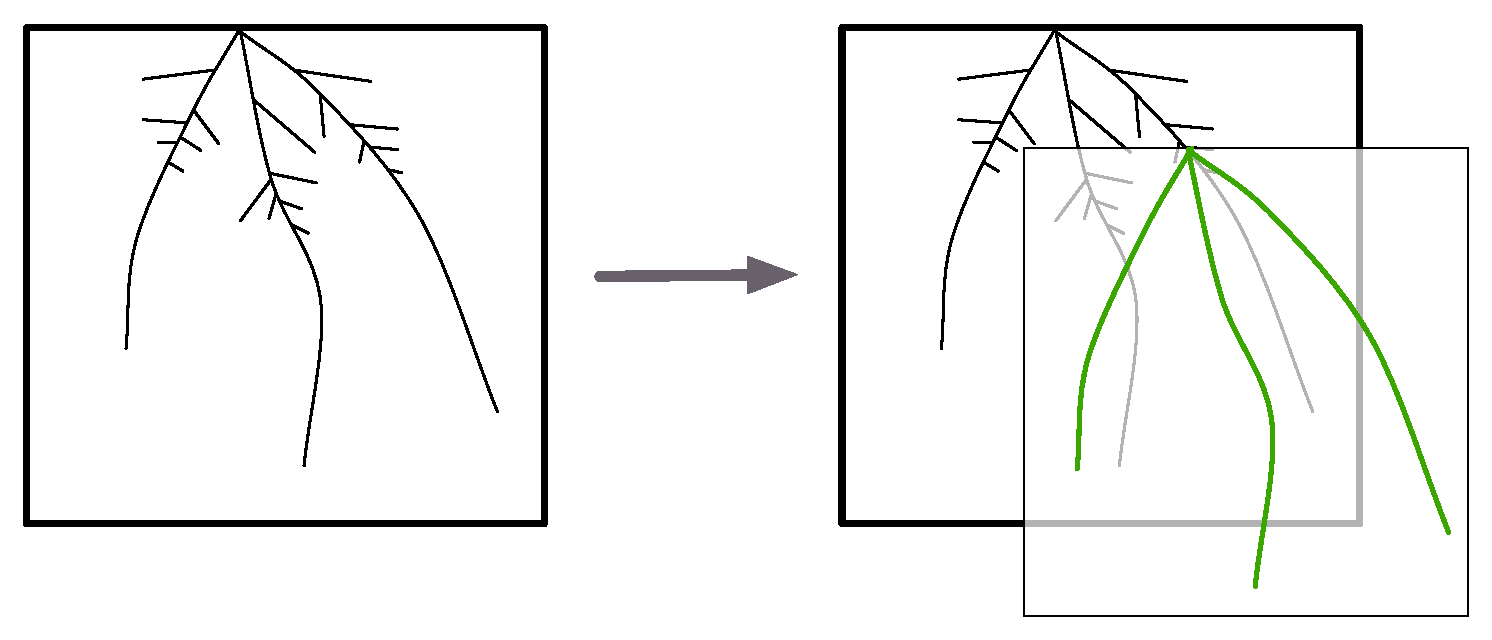
\includegraphics[width=0.6\linewidth]{insitu.pdf}
\caption[In situ drawing]{\textbf{In situ drawing.} Drawing of the axis of the root system inside the rhizotron}
\label{insitu}
\end{center}
\end{figure}


\section{Preparing the roots}

Take the roots out of the rhizotrons and wash them carefully. A soap bath and a brush can be used to ease the cleaning. If you do not want to directly scan your root system (for instance if you have several of rhizotron to unmount), store them either in clean water (for a few hours) or in FAA (for weeks if needed).\\


\section{Individual root scan}

Once the tracing is done, fix the root axis drawing at the bottom of the scanner (fig. \ref{scan}). It is better to use a flatbed scanner in which the roots are sitting in the water (fig. \ref{scanner}) in order to allow them to recover their initial shape.\\

For every root system you want to scan, cut the different root axis. For each of these root axis, replace it on the root drawing and scan it individually (fig. \ref{scan}). Because every root axis is different and because they tend to recover their initial shape in the water, replacing an axis on its drawing is relatively easy. Usually, lateral roots will keep their initial shape and angle in the water. If they are tangled, do not hesitate to use a brush the separate them. try to avoid root overlapping as much as possible.\\

For an optimal scanning procedure, use a 600 DPI resolution.\\

Be careful not to move the root axis drawing fixed at the bottom of the scanner. It is crucial that it does not move.\\

A the end of this procedure, you will end up with several $x$ scans by root system, $x$ being equal to the number of root axis (fig. \ref{scan}).  


\begin{figure}[htbp]
\begin{center}
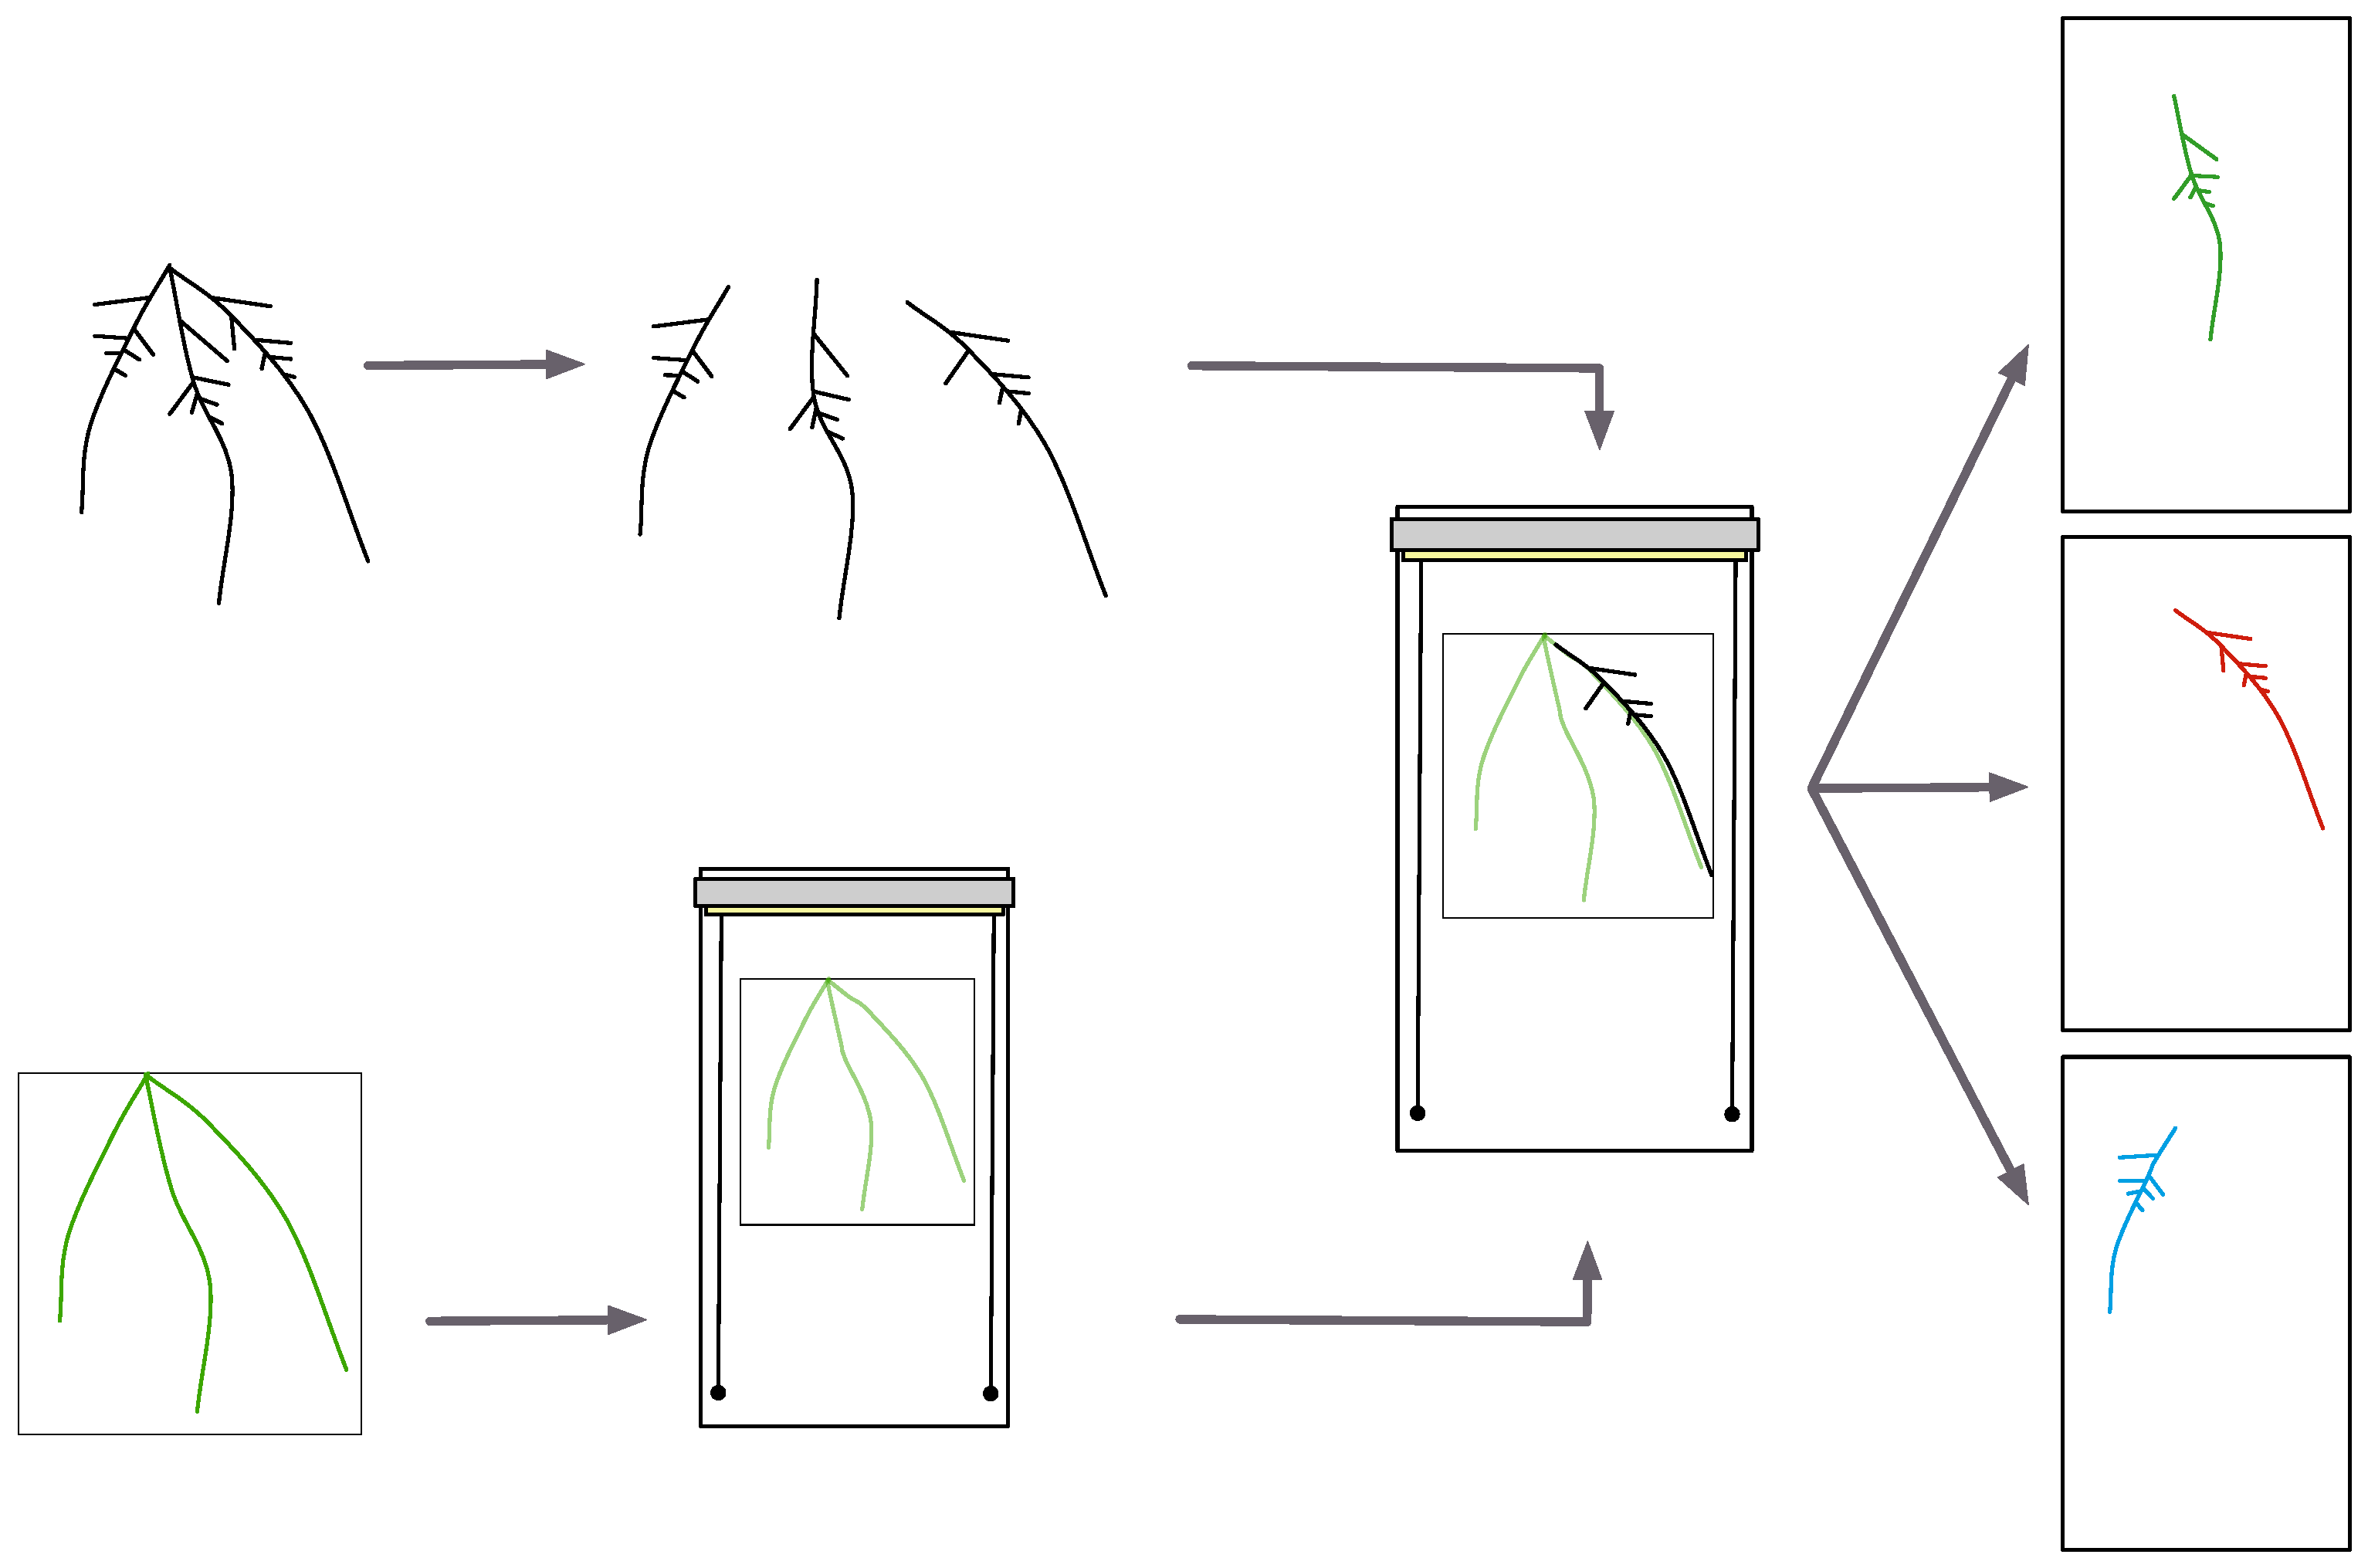
\includegraphics[width=0.7\linewidth]{scan.pdf}
\caption[Individual root scan]{\textbf{Individual root scan.} First the root axes drawing is fixed at the bottom of the scanner. Then, every root axes is replace on the axes drawing as it was inside the rhizotron and scanned separately.}
\label{scan}
\end{center}
\end{figure}

\begin{figure}[htbp]
\begin{center}
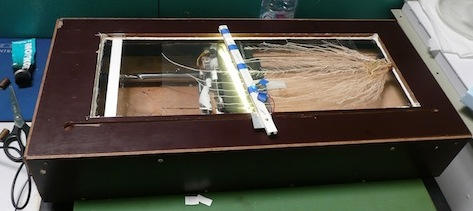
\includegraphics[width=0.65\linewidth]{scanner}
\caption[Root scanner]{\textbf{Root scanner} The scanning window can be submerge with water in order to easily spread the roots.}
\label{scanner}
\end{center}
\end{figure}

%%%%%%%%%%%%%%%%%%%%%%%%%%%%%%%%%%%%%%%%%%

\chapter{From scanned roots to digitalized structure}

\section{Principle}

Now that the roots are scanned, we would like to extract useful topological and morphological informations out of the scan. We also would like to be able to create a digital version of the root system.\\

To achieve these two goals, every root system will be analyzed with ImageJ \cite{Rasband11} and SmartRoot \cite{Lobet11}. The results of the different racing will be send to an unique data table (one data table per root system) (fig. \ref{numerisation}).\\

\begin{figure}[htbp]
\begin{center}
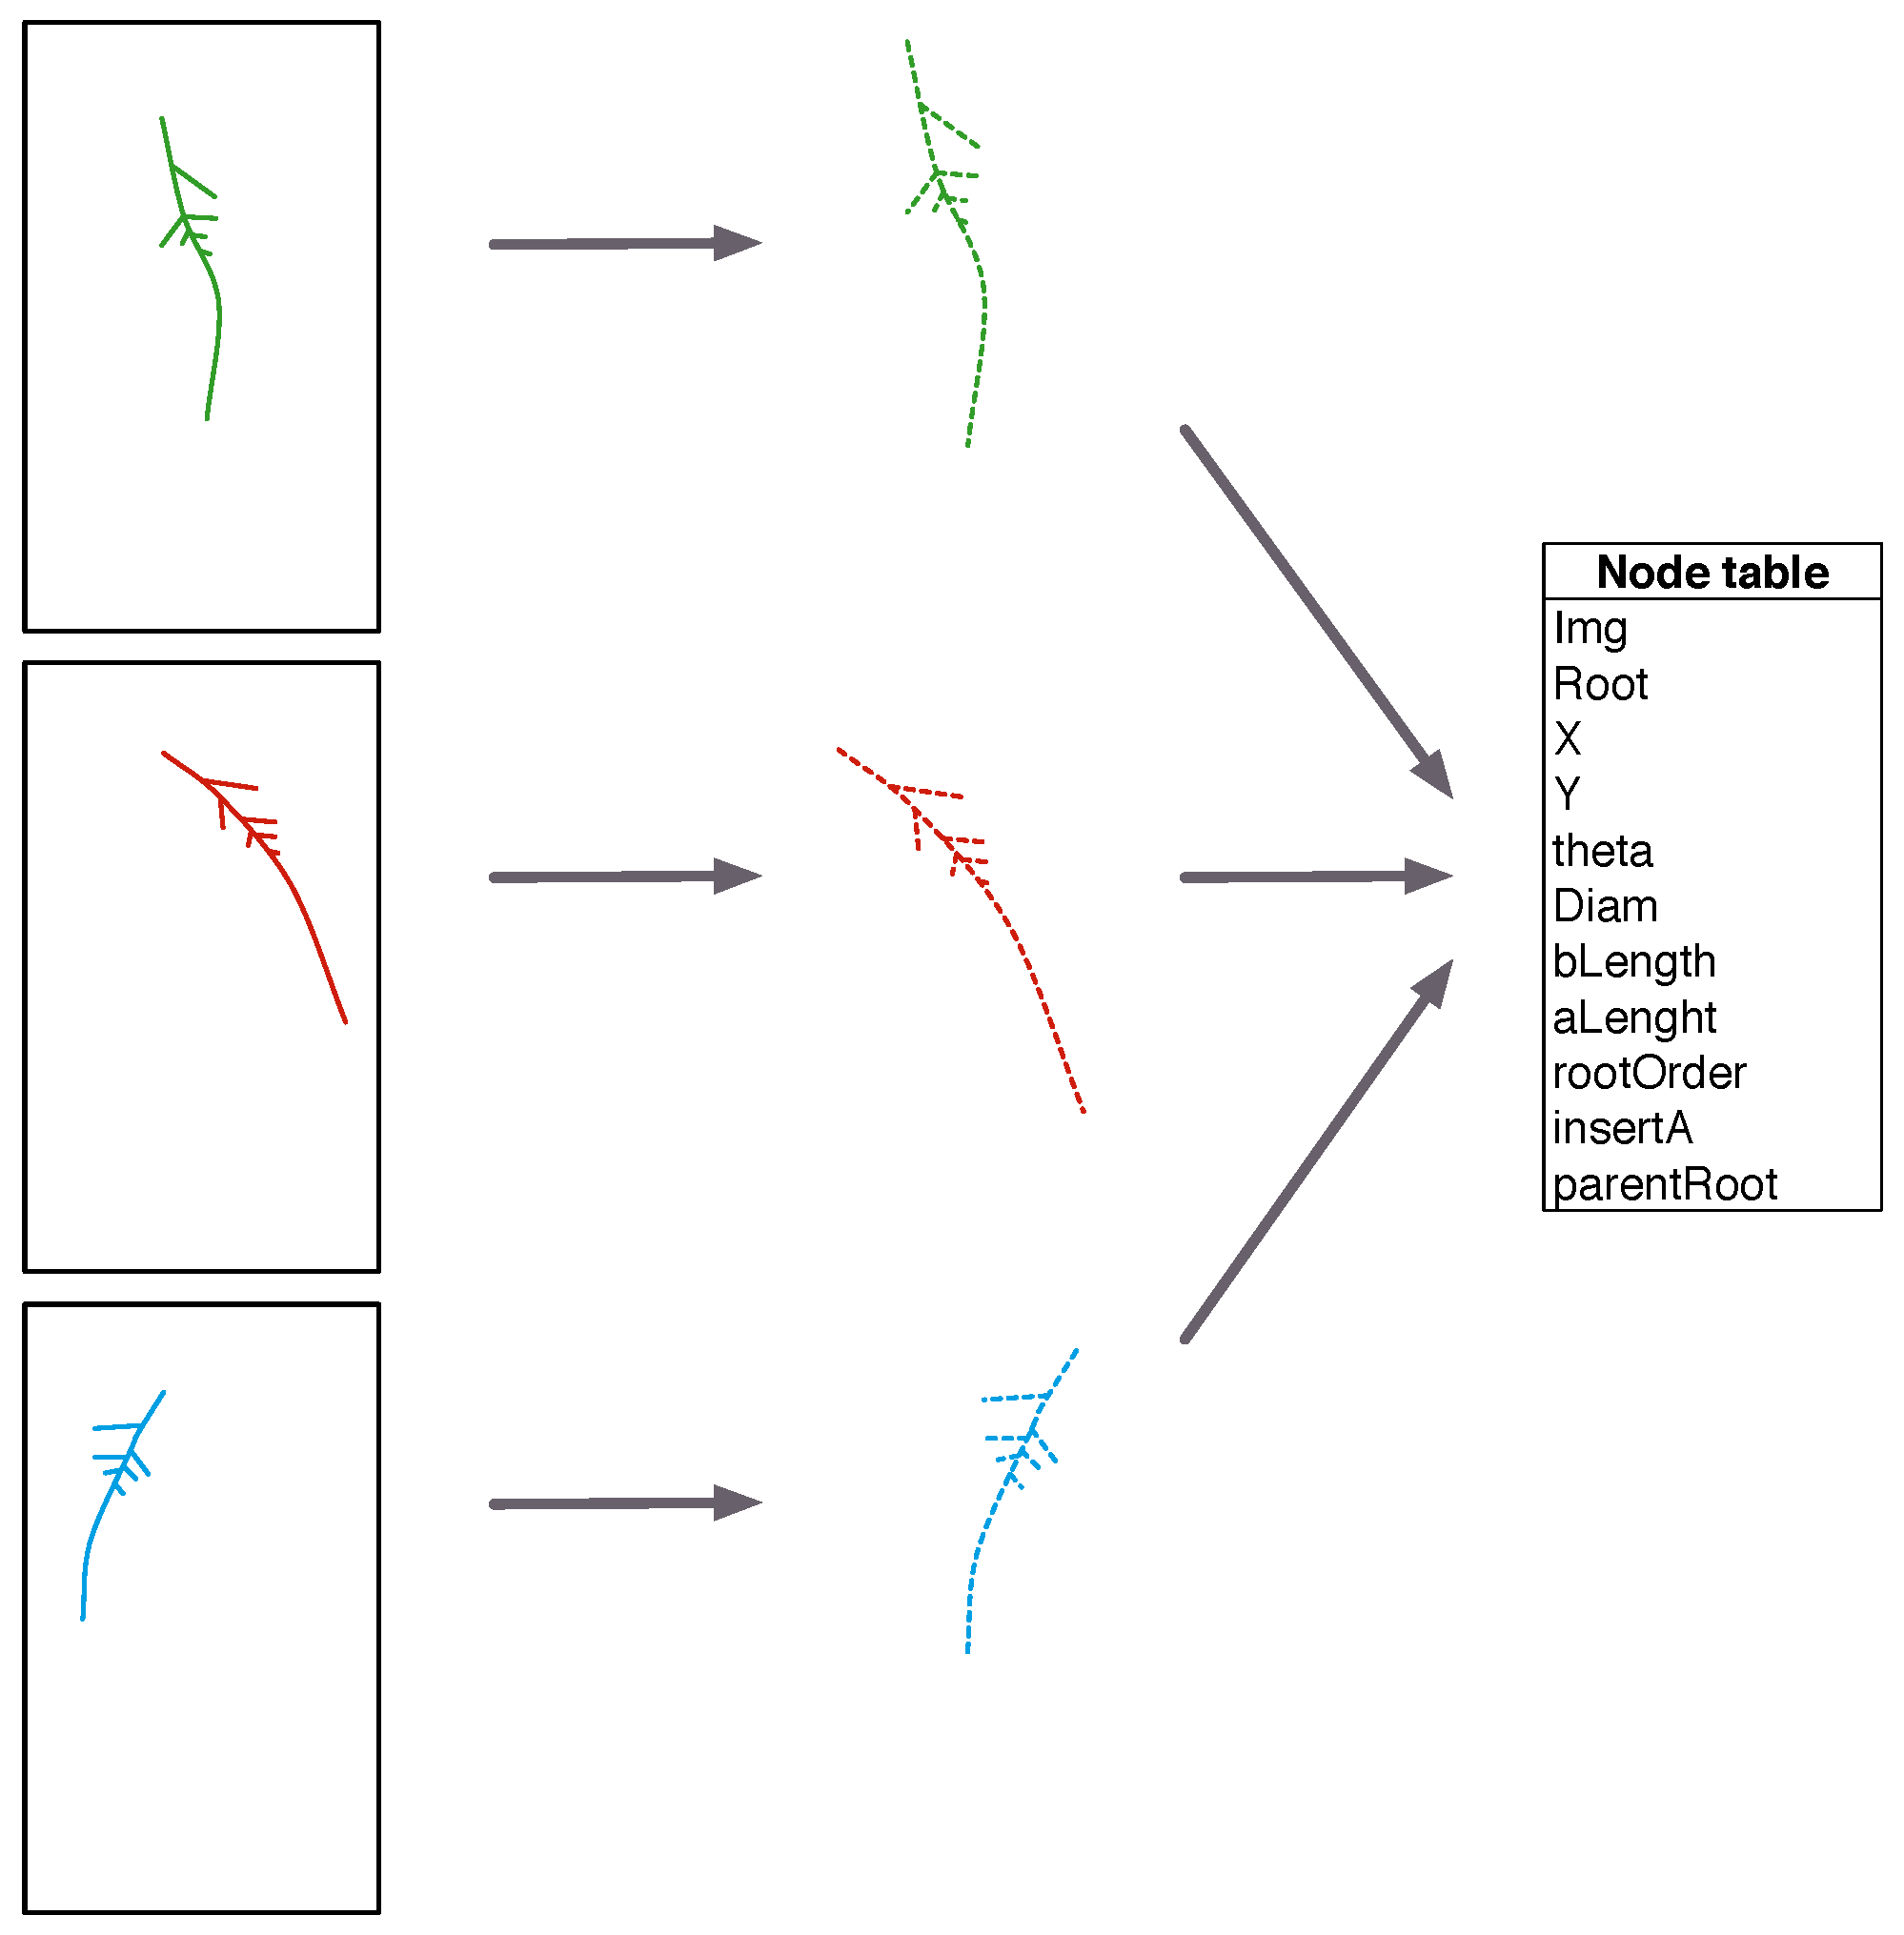
\includegraphics[width=0.7\linewidth]{numerisation.pdf}
\caption[Root numerisation.]{\textbf{Root numerisation.} Trace every axes with SmartRoot and export all the node data to a single data table.}
\label{numerisation}
\end{center}
\end{figure}


\section{Before tracing the roots}

Because the scan image size is not always the same as the size of the root drawing we will have to crop the different root scan before analyzing them.\\

\begin{enumerate}
\item Open ImageJ
\item Go to \verb|File > Import > Image Sequence| and choose the first scan of the root system
\item Make a rectangle selection which encompass the whole root drawing with top of the rectangle at the top of the drawing (fig. \ref{crop}).
\item Crop the image sequence (\verb|Image > Crop|)
\item Separate the sequence into individual images (\verb|Image > Stack > Stack to Images|) and save them.
\end{enumerate}

\begin{figure}[htbp]
\begin{center}
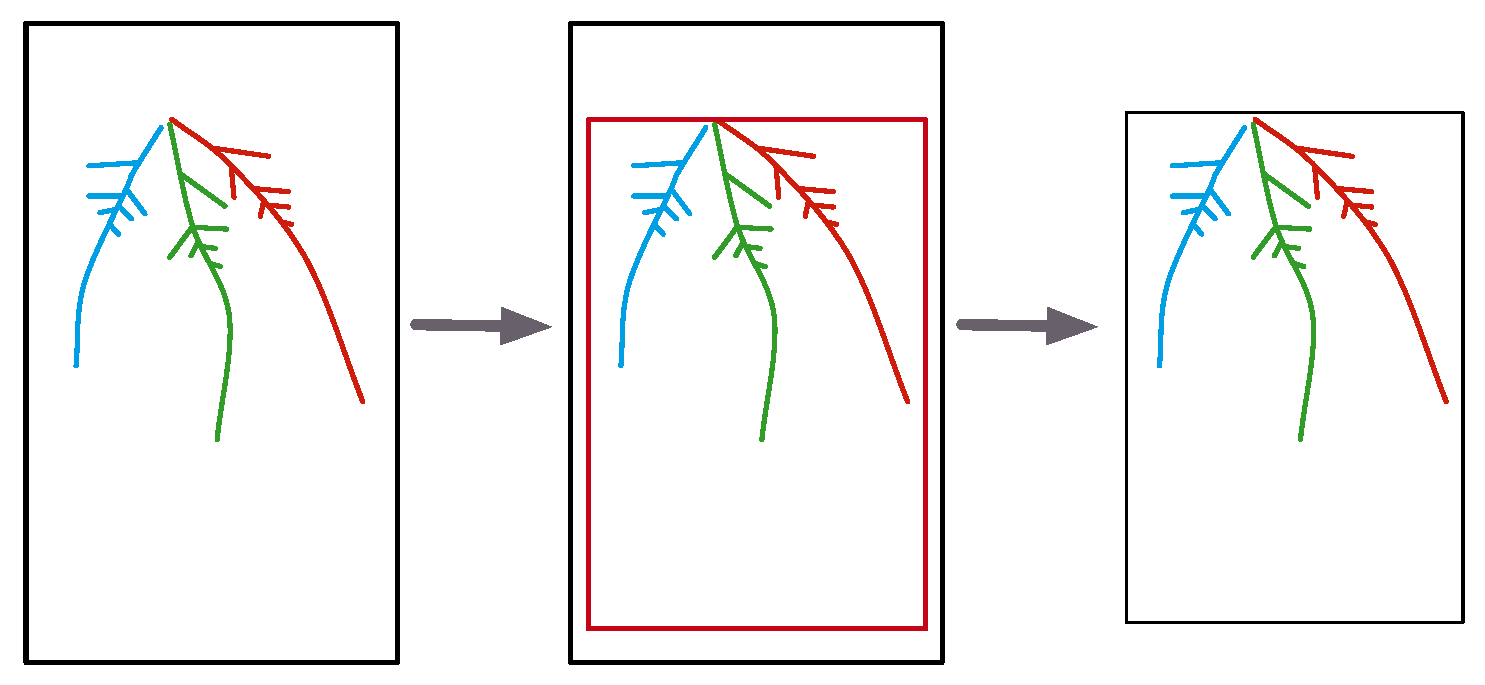
\includegraphics[width=0.5\linewidth]{crop.pdf}
\caption[Image crop]{\textbf{Image crop} Make a rectangle selection which encompass the whole root drawing with top of the rectangle at the top of the drawing. Crop the image image sequence}
\label{crop}
\end{center}
\end{figure}

\section{Tracing and exporting the roots}

Open SmartRoot and start tracing the root. For instruction about how to use SmartRoot, please refer to the user manual.\\

Some recommendations / tips for the tracing:

\begin{itemize}
\item Consider the root axis as the parent
\item Do not forget topology (attach laterals to their parent)
\item Use the \verb|Fast find Laterals| function to automatically trace lateral root.
\item For manually traced laterals, use the \verb|Root List| panel to attach them to their parent\\
\end{itemize}

One the root is traced, export it to your database (using the \verb|Data transfers| pane). \\

If you are exporting the first tracing of a root system, you have to create the data table. To do so, write down its name, check the \verb|Create a new table| button and select the \verb|Root Nodes| dataset. It is important that the name is in the form \textbf{{\color{red}EXP}$x${\color{red}\_R}$y${\color{red}\_N}}, where $x$ is the identifier of the experiment and $y$ the identifier of the rhizotron (has to be an integer). Click the \verb|Transfers| button to create the table and export the data\\

For the next tracing, use the same dataset and the same table name but uncheck the \verb|Create a new table| button. If this button stay checked, the new export will erase the previous ones.

%%%%%%%%%%%%%%%%%%%%%%%%%%%%%%%%%%%%%%%%%%


\chapter{From digitalized structure to R-SWMS input file}

Once the root system is digitalized, it is possible to retrieve the digitalized data and to use them to generate an R-SWMS input file. A small program, SRToRSWMS, was created to generate these input file. This program can generate the input files for all the rhizotron of one experiment at the same time.

\section{How to use the software}

\begin{itemize}
\item If you are on Windows, right click on the SRToRSWMS\_win.jar file and choose \verb|Open with > JavaTM (SE)..|
\item If you are on MacOS, double click on the SRToRSWMS\_mac.jar file.
\item A new window will open 
\item Fill the different fields:
	\begin{description}
	\item [Experience number:] Your experience identifier
	\item [Number of rhizotrons:] The number of rhizotrons in your experiement
	\item [Mean growth rate:] The mean root growth rate in cm/day
	\item[Driver:] the database driver name 
		\begin{description}
		\item[Microsoft Access:] sun.jdbc.odbc.JdbcOdbcDriver
		\item[MySQL:] com.mysql.jdbc.Driver
		\end{description}
	\item[Connection:] The connection info
		\begin{description}
		\item[Microsoft Access:] jdbc:odbc:
		\item[MySQL:] jdbc:mysql://localhost/
		\end{description}	
	\item[Name:] The database name
	\item[Username:] The connection username
	\item[Password:] The connection password
	\item[Output options:] Choose the output folder for the R-SWMS input files. 
	\end{description}
\item Hit the \verb|Run| button	
\end{itemize}
 

\newpage
\bibliography{/Users/guillaumelobet/documents/agro/doctorat/rapports/these.bib}


\end{document}  